\documentclass{beamer}

\usepackage{xcolor}
\usepackage{lmodern}
\usepackage{geometry}
\usepackage{calc}
\usepackage{textpos}
\usepackage{ragged2e}
\usepackage{hyperref}

\usepackage{cite}
\usepackage{amsmath}
\usepackage{xspace}
\usepackage{graphicx}
\usepackage{svg}
\usepackage{cleveref}
\usepackage{framed}
\usepackage{comment}
\usepackage{float}
\usepackage{rotating}
\usepackage{xstring}

\newcommand{\jx}{JX\xspace}
\newcommand{\extrafun}{JSON~eXtended\xspace}
\newcommand{\mf}{Makeflow\xspace}
\newcommand{\wq}{Work~Queue\xspace}
\newcommand{\lm}{Lifemapper\xspace}
\newcommand{\nd}{University of Notre~Dame\xspace}
\newcommand{\ndcity}{Notre~Dame, Indiana~46556\xspace}
\newcommand{\ccl}{ccl.cse.nd.edu\xspace}
\newcommand{\viz}{ccl.cse.nd.edu/software/workqueue/status\xspace}
\newcommand{\github}{github.com/cooperative-computing-lab/cctools\xspace}
\newcommand{\condor}{ND-Condor\xspace}
\newcommand{\jetstream}{IU-Jetstream\xspace}
%\newcommand{\batch}{Amazon-Batch\xspace}
\newcommand{\comet}{SDSC-Comet\xspace}
% we really don't need  ♭
\renewcommand{\flat}{Fine-Grained\xspace}
\newcommand{\nested}{Coarse-Grained\xspace}

%\newcommand{\svgpic}[1]{\begin{minipage}{\columnwidth}\begin{figure}[H]\centering\def\svgwidth{\columnwidth}\input{#1}\end{figure}\end{minipage}}

\geometry{a0paper,portrait,hmargin=2cm}
\usetheme{poster}
\usecolortheme{poster}

\begin{document}
\begin{frame}[fragile]
\frametitle{
  {\fontsize{64pt}{64pt}\selectfont
  \textbf{A First Look at the JX Workflow Language}} \\ \vspace{32pt}
  {\fontsize{48pt}{48pt}\selectfont
  Tim Shaffer, Kyle M.D. Sweeney, Nathaniel Kremer-Herman, and Douglas Thain}
}

\vspace*{64pt}

\begin{minipage}[t][0.97\textheight]{0.65\textwidth}
\begin{minipage}[t][0.86\textheight]{0.48\textwidth}

%\begin{block}{Abstract}
%Scientific workflows are typically expressed as a graph
%of logical tasks, each one representing a single program along with
%its input and output files.
%This poster introduces \jx~(\extrafun), a declarative language that
%can express complex workloads as an assembly of sub-graphs that
%can be partitioned in flexible ways.  We present a case study
%of using \jx to represent complex workflows for the \lm
%biodiversity project.  We evaluate partitioning approaches across several computing environments, including \condor, \jetstream, and \comet, and show that a coarse partitioning results in faster
%turnaround times, reduced data transfer, and lower master utilization
%across all three systems.
%\end{block}

\begin{alertblock}{Workflow Partitioning\rule{0pt}{2.1ex}}
\vspace*{16pt}
\parbox{\linewidth}{\emph{Workflow partitioning} is the process of splitting a workflow graph into sub-graphs,
such that each sub-graph will become a discrete
batch job in the target execution system.
The most appropriate partitioning depends on
many properties of the workflow graph,
such as the size of data objects and the execution
time of tasks, as well as the performance properties
of the execution system.}

\vspace*{32pt}

\fbox{
\raisebox{-0.5\height}{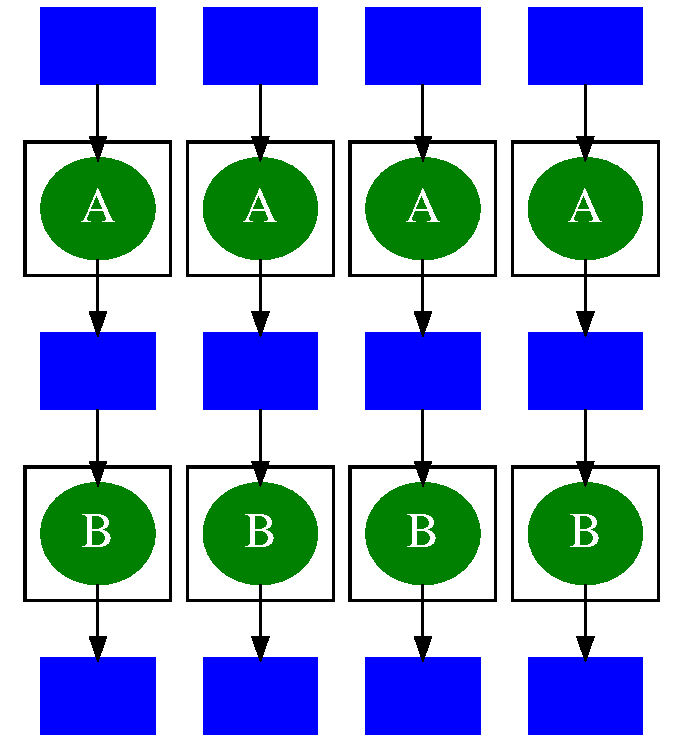
\includegraphics[width=0.48\linewidth]{figures/partition2.pdf}}
\hfill
\raisebox{-0.5\height}{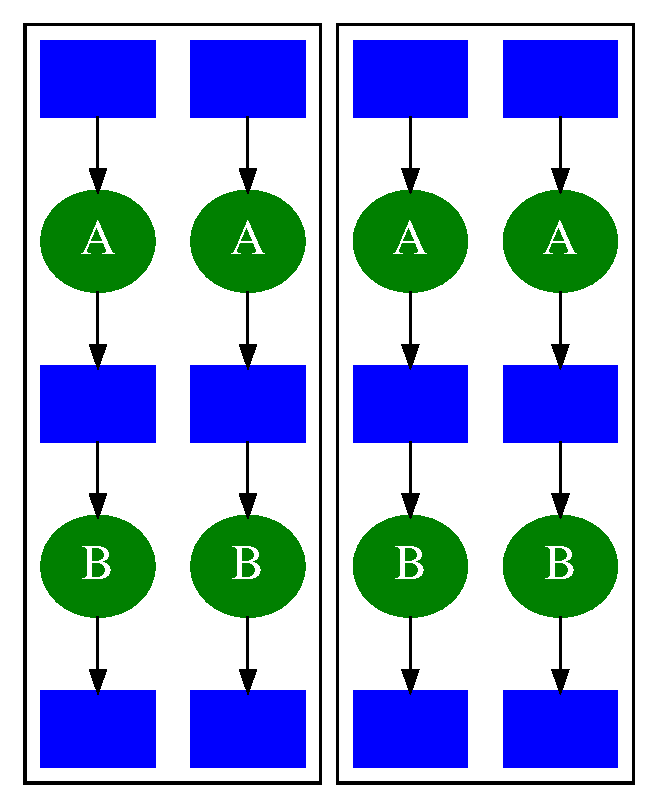
\includegraphics[width=0.48\linewidth]{figures/partition1.pdf}}}
\vspace{32pt}

\parbox{\linewidth}{On the left, a fine-grained scheme assigns each task to its own partition.
This is the most conservative approach,
and usually the default for workflow managers.
On the right,
coarser partitions group multiple tasks together.}
\end{alertblock}

\vfill

\begin{alertblock}{Evaluation\rule{0pt}{2.1ex}}
\vspace*{16pt}
\parbox{\linewidth}{We explored schemes for partitioning \lm, a distributed biodiversity modeling application.
As a high-throughput application,
\lm offers significant freedom in organizing computation beyond simply following data dependency relationships.
We observed that the granularity at which we distribute pieces of the workflow has a significant impact on its overall behavior.

\vspace{32pt}

We measured the behavior of \lm under two different partitioning schemes and ran the application on the \jetstream, \condor, and \comet{} execution sites.
We observed substantial differences in performance in terms of execution time, node-local storage, and data transfer between configurations when running on the same execution site.
Across all three computing sites,
there were similar trends in reduced data transfer and execution time with coarser workflow partitioning.}
\end{alertblock}

\vfill

\begin{alertblock}{Summary of Execution Sites\rule{0pt}{2.1ex}}
\vspace*{16pt}
\begin{center}
\begin{tabular}{|c|c c c c|}
\hline
           & Cores/ & Total  & Memory & Peak \rule{0pt}{2.1ex} \\
           & Worker & Cores  &        & Network \\ \hline
\condor    & 12     & $\sim$1200 & 20 GB  & 1 GB/s \rule{0pt}{2.1ex} \\
\jetstream &  10    & 110    & 30 GB  & 10 GB/s \\
\comet     & 12     & $\sim$1200 & 20GB   & InfiniBand \\
\hline
\end{tabular}
\end{center}
\end{alertblock}

\vfill

\begin{alertblock}{\lm queries at three different scales\rule{0pt}{2.1ex}}
\vspace*{16pt}
\parbox{\linewidth}{In each diagram,
boxes represent files with arrows connecting to tasks,
represented as ovals.
Here \textbf{Q} denotes query data,
\textbf{T} denotes tools such as Python scripts and Java JAR files,
\textbf{R} denotes common reference data,
and \textbf{D} denotes output data.
The upper left workflow shows a small query against a single data layer for the \textit{Heuchera} data set.
The next workflow to the right shows a larger query against the \textit{Saxifragales} data set with three data layers.
Below, we duplicated layers to create a twelve-layered query against \textit{Saxifragales}.}

\vspace{32pt}

\raisebox{-0.5\height}{\fbox{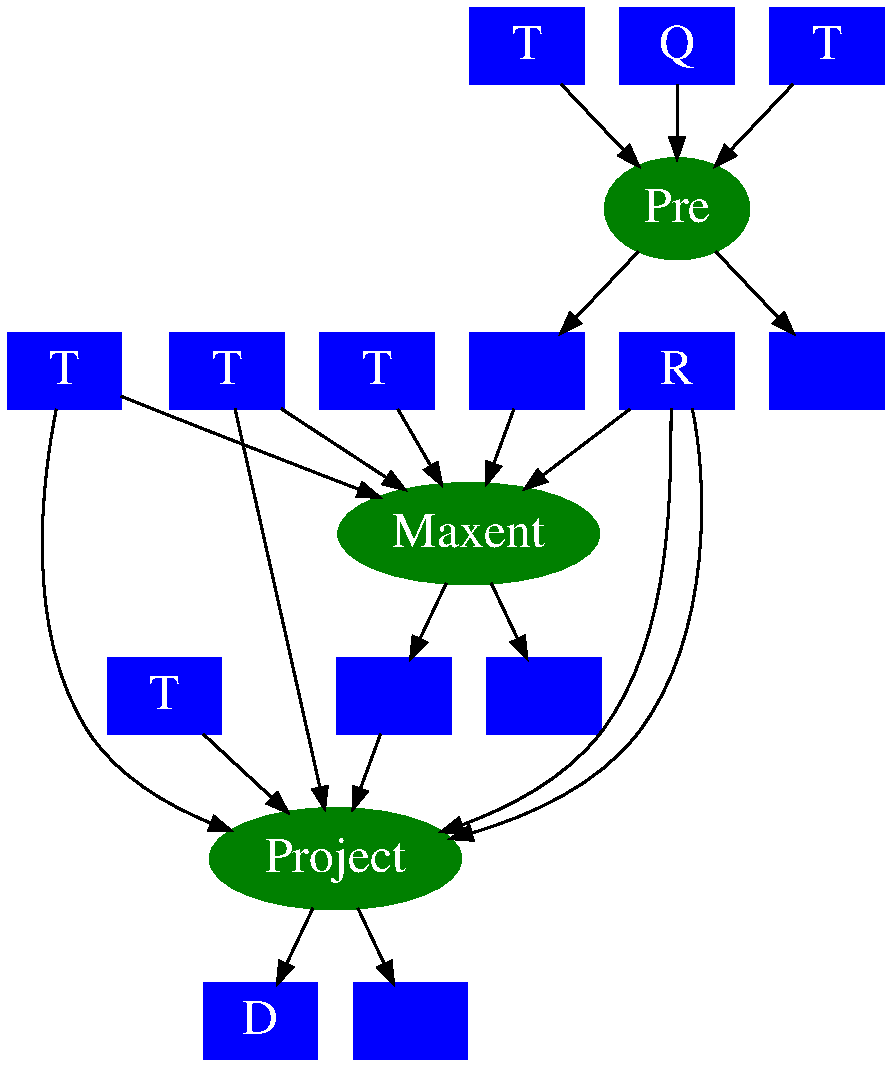
\includegraphics[width=0.37\linewidth]{figures/small.pdf}}}
\hfill
\raisebox{-0.5\height}{\fbox{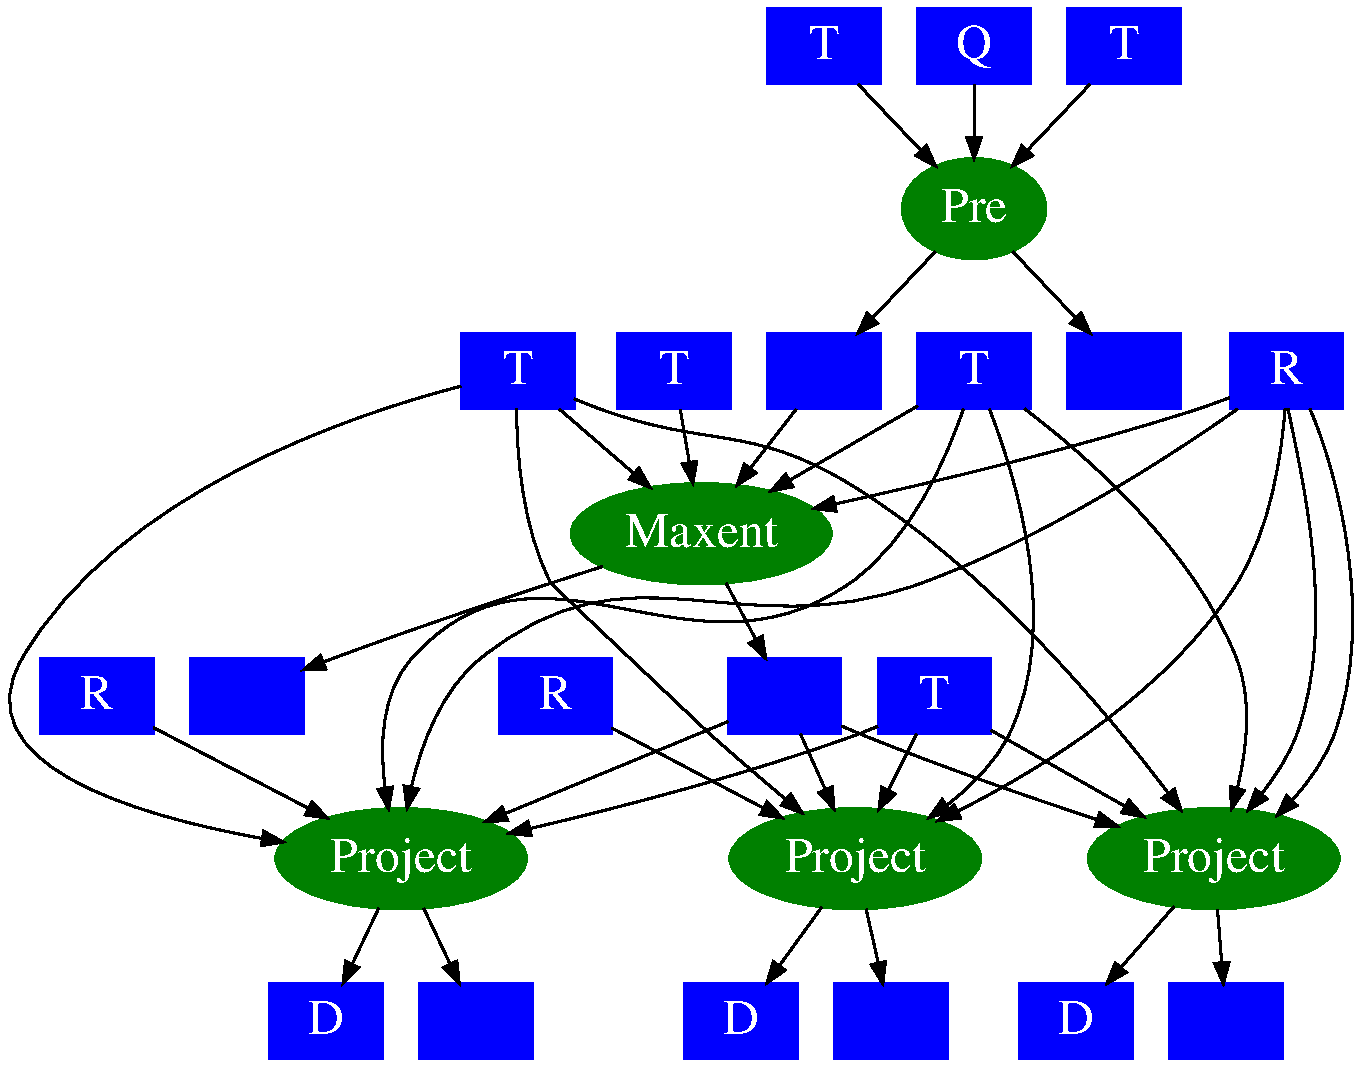
\includegraphics[width=0.56\linewidth]{figures/large.pdf}}}
\end{alertblock}

\end{minipage}\hfill
\begin{minipage}[t][0.85\textheight]{0.48\textwidth}

\begin{alertblock}{Partitioning Schemes for Lifemapper\rule{0pt}{2.1ex}}
\vspace*{16pt}
\parbox{\linewidth}{These simplified workflows consist of four small taxa.
The labels have the same meaning as above.
Unlabeled boxes are intermediate files that are discarded after the workflow completes.
With the \flat configuration,
There is no additional structure within the workflow beyond data dependencies.
With the \nested configuration,
The taxa are arranged into two partitions.
Each partition becomes a task in the high level workflow.}

\vspace{16pt}

\fbox{\parbox{\linewidth}{\centering
\vspace*{16pt}
\textbf{\flat Model} 
\vspace{16pt}

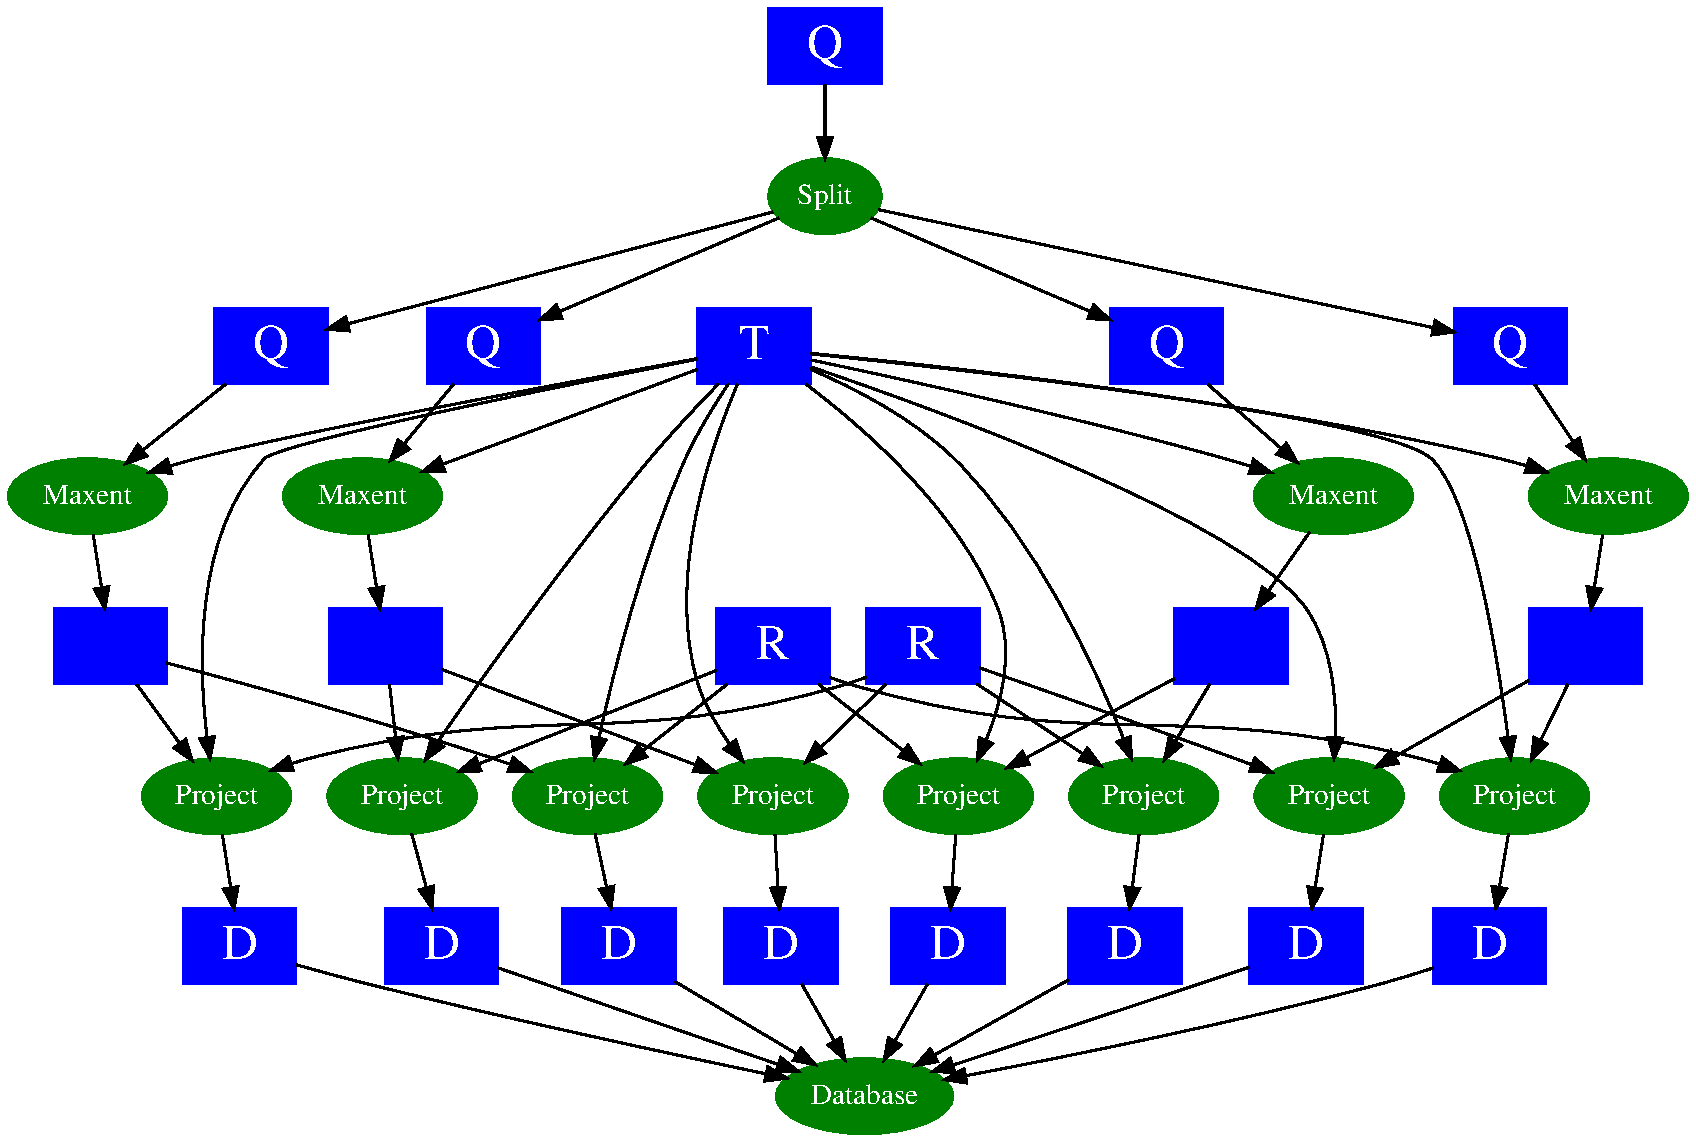
\includegraphics[width=.75\linewidth]{figures/flat.pdf}
\vspace*{16pt}}}

\vspace{16pt}

\fbox{\parbox{\linewidth}{\centering
\vspace*{16pt}
\textbf{\nested Model}
\vspace{16pt}

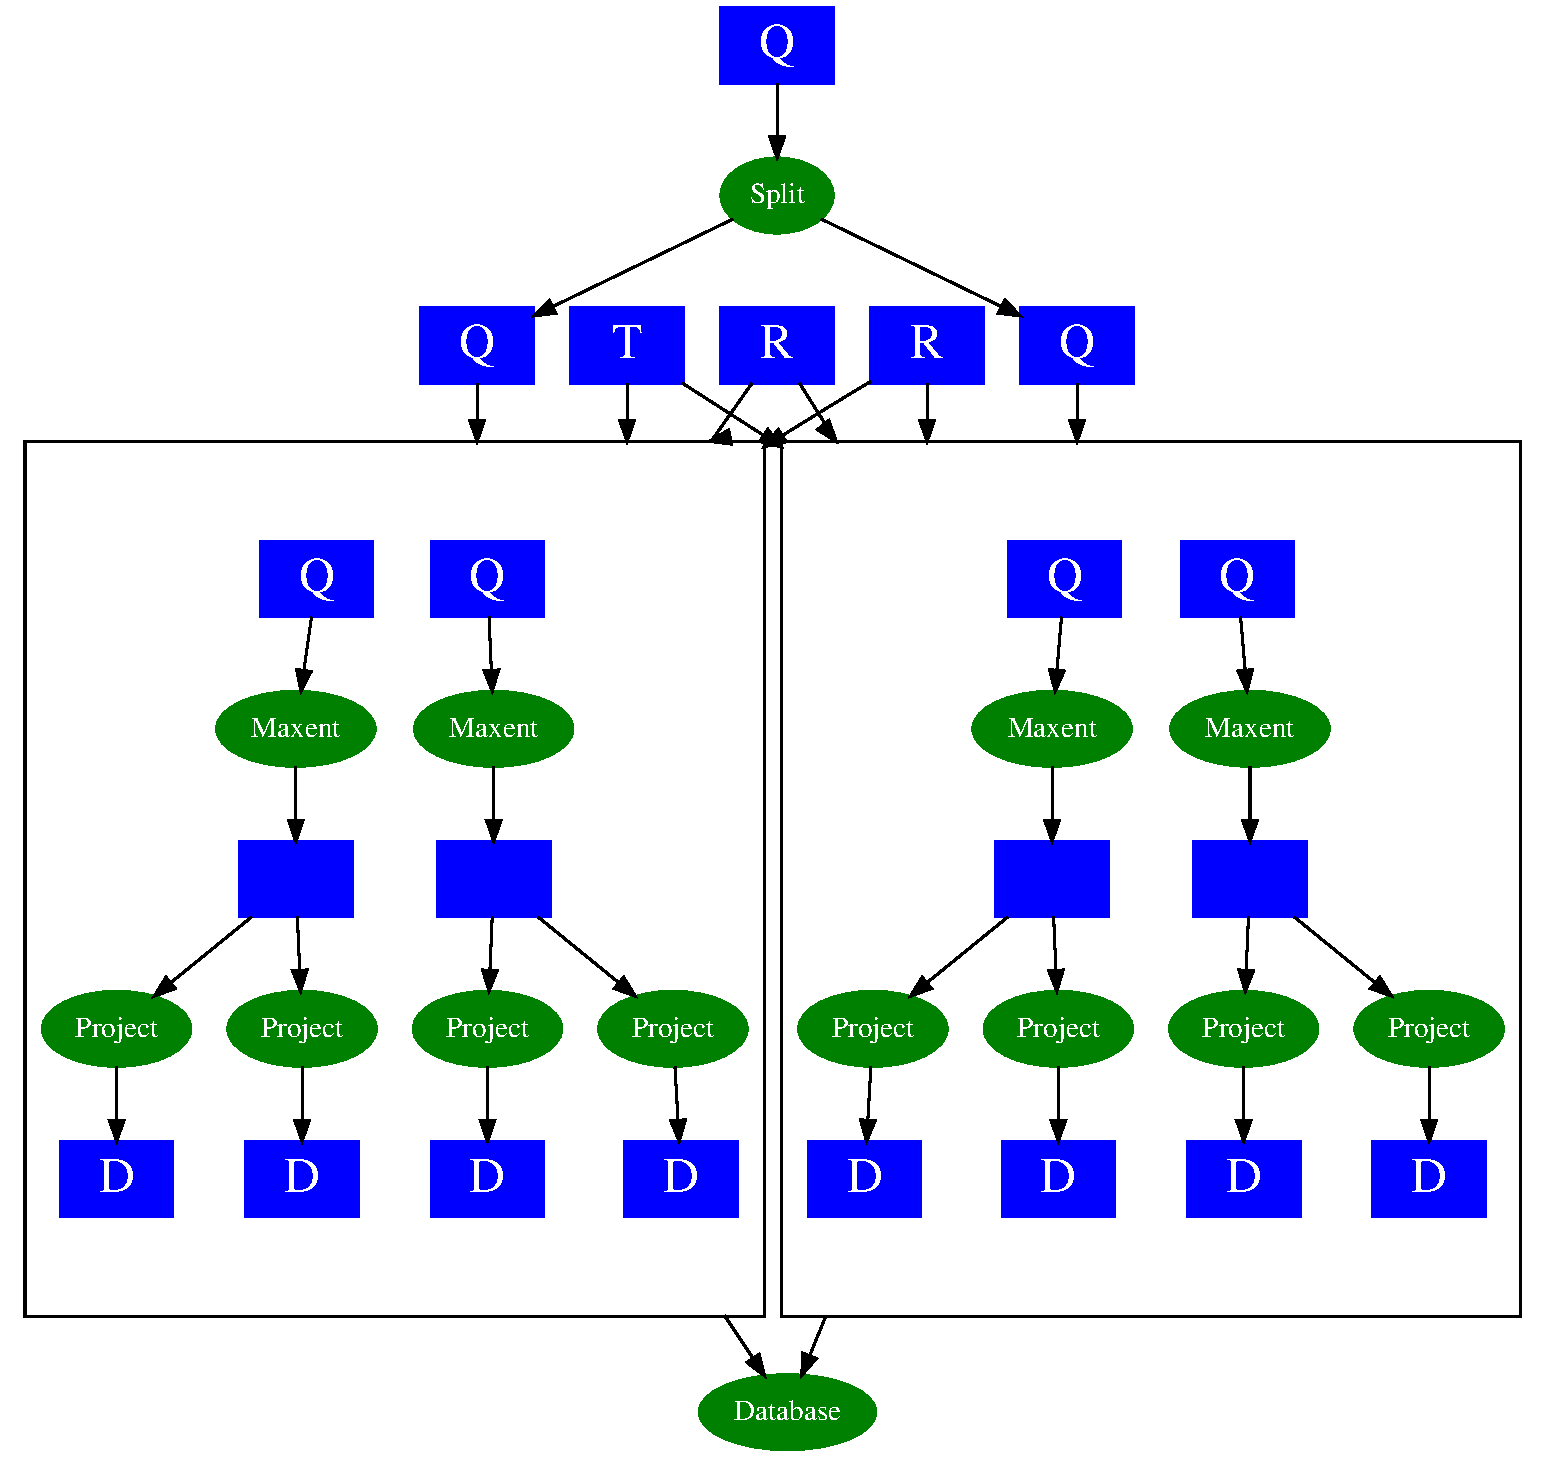
\includegraphics[width=.75\linewidth]{figures/nested.pdf}
\vspace*{16pt}}}
\end{alertblock}

\vfill

\begin{alertblock}{\jx: \extrafun\rule{0pt}{2.1ex}}
\vspace*{16pt}
\parbox{\linewidth}{We developed \jx~(\extrafun) as a language for expressing workflows that allows for easy manipulations to the structure and partitioning of a workflow.
\jx extends a JSON representation of the workflow by supporting a subset of Python expressions,
allowing for a concise intermediate representation that expands to a normal JSON document.
Templates in \jx can expand to complicated nested workflow structures based on parameters,
allowing flexible changes to a workflow's partitioning scheme.

\vspace{16pt}

The following workflow ``template'', when expanded,
expresses an entire map-reduce type workflow.
The expanded workflow includes a rule for each of the $N$ input files,
and a reduce step that takes all $N$ intermediate files and produces the final output.
This template exposes the structure of the workflow as a parameter.
These parametric templates are the primary way \jx allows for flexible changes in the organization and partitioning scheme of a scientific workflow.}
\end{alertblock}

\vfill

\begin{exampleblock}{Complete JX Workflow\rule{0pt}{2.1ex}}
\begin{verbatim}
{
  "rules": [{
    "inputs":
      ["split." + str(i)],
    "outputs":
      ["out." + str(i)],
    "command":
      "./process.sh split." + str(i),
  } for i in range(N)] + [{
    "inputs":
      ["out." + str(i) for i in range(N)],
    "outputs":
      ["result.dat"],
    "command":
      "./reduce.sh out.*",
  }]
}
\end{verbatim}
\end{exampleblock}

\vfill

\end{minipage}

\begin{block}{}
\begin{center}
\fbox{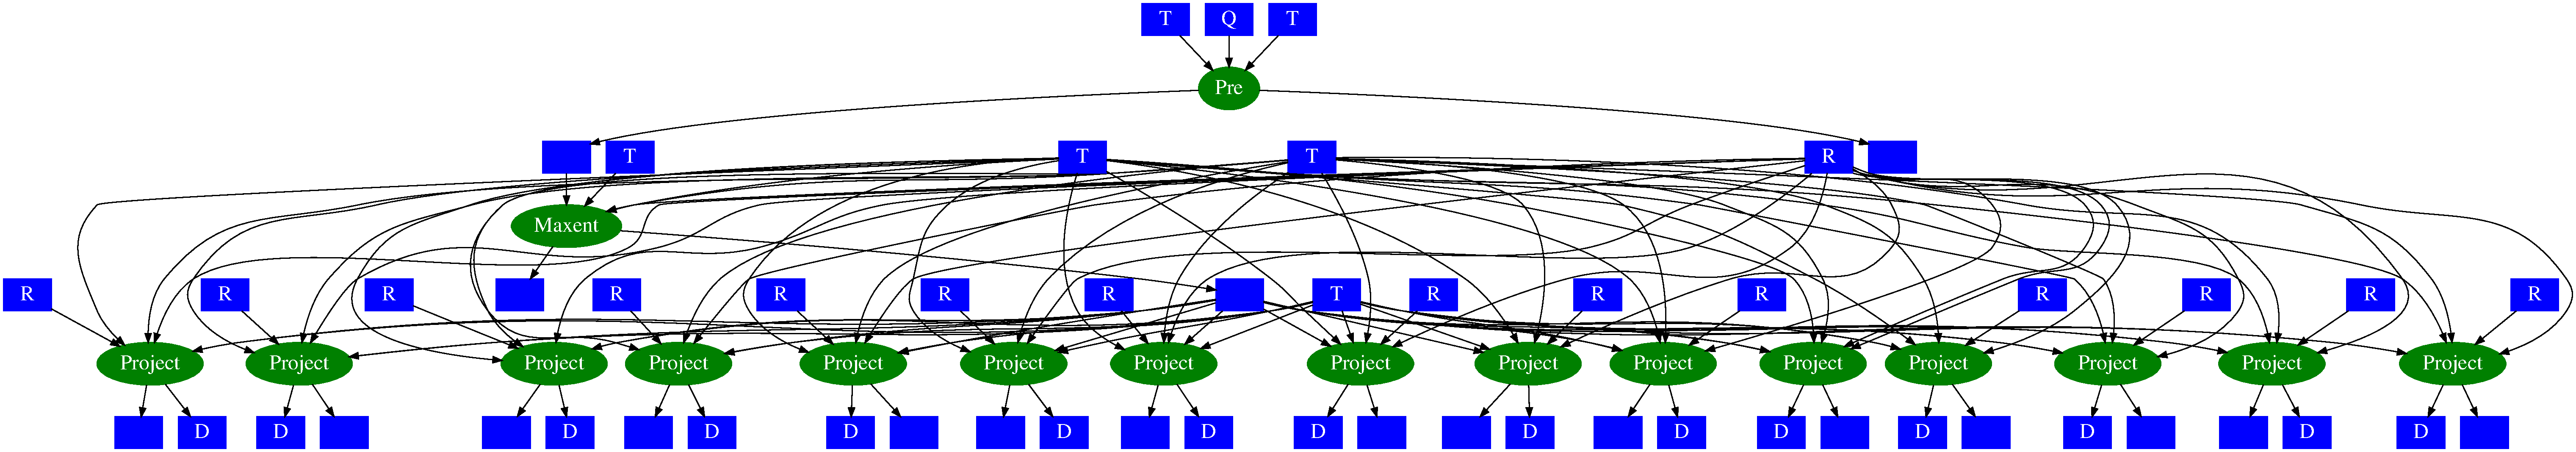
\includegraphics[width=\linewidth]{figures/huge.pdf}}
\end{center}
\end{block}

\end{minipage}\hfill
\begin{minipage}[t][0.95\textheight]{0.33\textwidth}

\begin{exampleblock}{Make Rule\rule{0pt}{2.1ex}}
\begin{verbatim}
proj/I_japonica.asc: I_japonica.csv
    ./project.sh I_japonica.csv proj
\end{verbatim}
\end{exampleblock}

\begin{block}{}
\parbox{\linewidth}{The GNU Make format is well-known, compact, and easy for novices to write, but it has some syntactic limitations.
It is also difficult to add additional data or fields to a rule
in a programmatic way, which is needed to handle partitioning and other
workflow transformations.
A JSON representation is easier to generate and parse via script,
but still very verbose.}
\end{block}

\begin{exampleblock}{Single Task Expressed in JSON\rule{0pt}{2.1ex}}
\begin{verbatim}
{
  "inputs": ["I_japonica.csv"],
  "outputs": ["proj/I_japonica.asc"],
  "command":
    "./project.sh I_japonica.csv proj"
}
\end{verbatim}
\end{exampleblock}

\vfill

\begin{block}{}
\parbox{\linewidth}{An entire workflow could be expressed as a sequence of plain                    
JSON records like the above.
\jx expands upon JSON to allow compact patterns to expand into JSON rules.
\jx supports variable substitutions when expanding a document,
multiple data types such as numbers and lists,
and common operators such as arithmetic and comparison.
These operators function the same as in Python.}
\end{block}

\begin{exampleblock}{JX Rule with Variable Substitutions\rule{0pt}{2.1ex}}
\begin{verbatim}
{
  "inputs": [s + ".csv"],
  "outputs": ["proj/" + s + ".asc"],
  "command":
    "./project.sh " + s + ".csv proj",
}
\end{verbatim}
\end{exampleblock}

\vfill

\begin{block}{}
\parbox{\linewidth}{To quickly generate a list of items
(e.g. a range of outputs like \texttt{file.1} \dots  \texttt{file.n}),
\jx supports Python-style list comprehensions.
For \texttt{SAMPLES = ["I\_japonica", "A\_arboreum"]},
we can produce a pair of rules,
one for each sample.}
\end{block}

\begin{exampleblock}{JX List Comprehension for Rules\rule{0pt}{2.1ex}}
\begin{verbatim}
[{
  "inputs": [s + ".csv"],
  "outputs": ["proj/" + s + ".asc"],
  "command":
    "./project.sh " + s + ".csv proj",
} for s in SAMPLES]
\end{verbatim}
\end{exampleblock}

\vfill

\begin{block}{}
\parbox{\linewidth}{Since the connections between tasks in a workflow (inputs and outputs) are specified as lists,
this gives substantial freedom in programmatically defining the structure of a workflow.
In addition, the workflow itself is primarily a list of rules,
making it possible to expand a large number of rules from a single template.
As an example, consider a workflow that takes an input file (\texttt{INPUT}),
splits it into \texttt{N} pieces,
and runs a processing script on each.}
\end{block}

\begin{exampleblock}{JX Workflow Template\rule{0pt}{2.1ex}}
\begin{verbatim}
{
  "rules": [{
    "inputs": [INPUT],
    "outputs":
      ["split." + str(i) for i in range(N)],
    "command": "./split.sh " + INPUT,
  }] + [{
    "inputs": ["split." + str(i)],
    "outputs": ["out." + str(i)],
    "command":
      "./process.sh split." + str(i),
  } for i in range(N)]
}
\end{verbatim}
\end{exampleblock}

\vfill

\begin{block}{}
\parbox{\linewidth}{Combining these features,
\jx allows us to treat a sub-workflow as a job.
A \jx template serves to define the structure of the sub-workflow subject to some parameters.
We can reuse the same definition to programmatically produce a large number of rules that fit the concrete arguments to each invocation.
We can pass the chosen partitioning into the high-level workflow,
which can then repeatedly expand the partition template and produce each sub-workflow as it is executed.
The following shell command could be a rule in the \mf workflow management system which expands the previous example template and runs the resulting workflow as a task.}
\end{block}

\begin{exampleblock}{Invoking Makeflow Using a JX Template\rule{0pt}{2.1ex}}
\begin{verbatim}
makeflow --jx-define 'INPUT="heuchera"' \
         --jx-define N=100 \
         template.jx
\end{verbatim}
\end{exampleblock}

\vfill

\begin{alertblock}{Acknowledgments}
Visit \url{http://ccl.cse.nd.edu/} to learn more!

This work was supported in part by National Science Foundation grant~OCI-1148330.
\end{alertblock}

\end{minipage}
\end{frame}
\end{document}
